\documentclass[10pt,letterpaper]{article}

\usepackage[margin=1in]{geometry}
\usepackage{amsmath,amssymb}
\usepackage{graphicx}
\usepackage{float}
\usepackage{booktabs}
\usepackage{array}
\usepackage{parskip}
\usepackage{fancyhdr}
\usepackage{enumitem}
\usepackage{hyperref}
\usepackage{xcolor}
\usepackage{parskip}
\usepackage{minted, mdframed}
\usepackage{hyperref}
\hypersetup{
colorlinks=true,
linkcolor=blue, %purple
citecolor= blue,
urlcolor=cyan
}

\usepackage[utf8]{inputenc}
\usepackage{tikz}
% \usetikzlibrary{shapes.geometric, arrows.meta, calc, positioning}
\usetikzlibrary{arrows.meta, calc, positioning, shapes.gates.logic.US, shapes.geometric}


\pagestyle{fancy}
\fancyhf{}
\lhead{CS M151A: Introduction to Digital Design Lab}
\rhead{Lab 2 - Floating Point Conversion}
\cfoot{\thepage}

\newcommand{\unit}[1]{\text{ #1}}

\title{\textbf{Lab 2 - Floating Point Conversion}}
\author{Don D. Le and Gaurav Kumar}
\date{Spring 2026}

\begin{document}

\maketitle
\tableofcontents
\listoffigures
\addcontentsline{toc}{section}{\listfigurename}
\clearpage

% ============================================================


\section{Introduction and Requirements}

This lab focuses on the design of a combinational circuit that converts a 12-bit signed integer in two's complement format into an 8-bit floating point representation with fields \texttt{S}, \texttt{E[2:0]}, and \texttt{F[3:0]}. Unlike Lab 1, this assignment is simulation-only, so the emphasis is on correct combinational behavior, careful treatment of edge cases, and thorough verification against representative test vectors.

\textbf{Lab objective.} The objective of this lab is to design and simulate a Verilog module that compresses a 12-bit two's complement input \texttt{D[11:0]} into an 8-bit floating point representation of the form $V = (-1)^S \times F \times 2^E$. To do this correctly, the circuit must extract the sign, convert negative values to magnitude before processing, generate a normalized significand and exponent from the input magnitude, and apply rounding based on the fifth bit following the leading 1. The design must also handle edge cases carefully, including significand overflow during rounding and saturation to the largest representable floating point value when the exponent would otherwise exceed its 3-bit range.

\textbf{Design requirements.} The floating point converter is required to accept a 12-bit input in two's complement form and produce the corresponding sign, exponent, and significand fields of the 8-bit floating point output. The sign bit must reflect the polarity of the original input, while negative values must first be converted to magnitude before any leading-zero counting or significand extraction is performed. The exponent must be determined from the number of leading zeroes in the magnitude according to the mapping specified in the handout, and the significand must be formed from the four bits immediately following the first significant 1, or from the least significant four bits when the exponent is zero. 

The design must also implement rounding to the nearest representable floating point value by examining the fifth bit after the leading 1, rounding down when that bit is 0 and rounding up when it is 1. Finally, the converter must correctly handle overflow cases by renormalizing the significand when rounding produces \texttt{10000} and by saturating to the largest representable floating point value when the exponent would exceed its maximum value.

\section{Design Description}

This section should document the implementation at the module level and explain how the Verilog design maps to the algorithm described in the lab handout.

\subsection{Top-Level Module Overview}

The design is implemented in \texttt{FPCVT.v} as a combinational module with one 12-bit input and three outputs:

\begin{itemize}
    \item \texttt{D[11:0]}: signed input in two's complement,
    \item \texttt{S}: sign bit of the floating point result,
    \item \texttt{E[2:0]}: 3-bit exponent,
    \item \texttt{F[3:0]}: 4-bit significand.
\end{itemize}

The overall dataflow in the implementation follows the same sequence as the handout. The input sign is first separated from the input word, and the remaining processing is performed on a magnitude value stored in \texttt{mag}. The magnitude then passes through a leading-zero detection stage that determines how far the value must be shifted for normalization and, equivalently, what exponent should be produced. After normalization, the design extracts four significand bits plus one additional rounding bit, then performs a final correction step to round the result and handle any overflow in the significand or exponent fields.

\subsection{Sign and Magnitude Conversion}

The sign output is generated directly from the most significant input bit by the assignment \texttt{S = D[11]}. The remaining logic works on an unsigned magnitude signal \texttt{mag}. If the input is nonnegative, the code simply copies \texttt{D} into \texttt{mag}. If the input is negative, the code computes the two's complement by inverting the bits and adding 1, which produces the absolute value needed for the floating point conversion steps. The one exceptional case is \texttt{D = 100000000000}, which corresponds to $-2048$. Since $+2048$ cannot be represented in 12 bits, the code explicitly maps this case to \texttt{011111111111}, effectively treating it like the largest positive magnitude that can still be processed by the rest of the design.

\subsection{Leading Zero Detection and Exponent Generation}

The leading-zero detection is implemented with a combinational \texttt{for} loop that scans the magnitude from bit 11 down to bit 0. A flag named \texttt{found} ensures that only the first \texttt{1} encountered is used. Once that bit position is found, the code computes \texttt{zeros = 11 - i}, which records how many leading zeroes appear before the most significant \texttt{1}. This value is then used to generate the exponent. Inputs with many leading zeroes produce small exponents, while large magnitudes with few leading zeroes produce larger exponents.

\begin{table}[H]
    \centering
    \caption{Fill-in summary of exponent encoding}
    \begin{tabular}{cc}
        \toprule
        Leading zeroes & Exponent \\
        \midrule
        1 & 7 \\
        2 & 6 \\
        3 & 5 \\
        4 & 4 \\
        5 & 3 \\
        6 & 2 \\
        7 & 1 \\
        $\geq 8$ & 0 \\
        \bottomrule
    \end{tabular}
    \label{tab:exp-map}
\end{table}

In the Verilog implementation, the exponent logic is expressed directly with a few cases. If \texttt{zeros >= 8}, the exponent is forced to \texttt{000}, which matches the low-magnitude rule from the handout. If \texttt{zeros == 0}, the exponent is set to \texttt{111}. For all other nonzero magnitudes, the code uses \texttt{E = 8 - zeros}, which reproduces the table above. This makes the exponent generation compact while still matching the required mapping between leading-zero count and encoded exponent.

\subsection{Significand Extraction and Normalization}

After the number of leading zeroes is known, the code normalizes the magnitude by left-shifting it by \texttt{zeros} positions and storing the result in \texttt{norm}. This places the first significant \texttt{1} at the most significant position of the shifted word. The design then extracts \texttt{norm[11:7]} into \texttt{frac\_ext}, where the upper four bits represent the candidate significand and the fifth bit is reserved for rounding. In normalized cases, this means the significand begins with the first significant \texttt{1}, which matches the preferred representation described in the handout. For small values where the exponent is 0, this same shift-and-slice approach still causes the lower-magnitude bits to be carried into the four-bit field, which is consistent with the low-range behavior expected by the assignment.

\subsection{Rounding Logic}

The rounding rule in the design follows the handout exactly: the fifth bit after the leading \texttt{1} decides whether the value rounds down or rounds up. In the implementation, \texttt{frac\_ext[4:1]} holds the four candidate significand bits, and \texttt{frac\_ext[0]} is the rounding bit. If \texttt{frac\_ext[0] = 0}, the code truncates and assigns \texttt{F = frac\_ext[4:1]}. If \texttt{frac\_ext[0] = 1}, the code adds 1 to the four-bit significand using the temporary signal \texttt{rounded}. Using a 5-bit intermediate value makes the logic straightforward because the same addition both performs the round-up operation and exposes whether a carry-out occurred.

\begin{table}[H]
    \centering
    \caption{Fill-in rounding examples}
    \begin{tabular}{ccc}
        \toprule
        Linear encoding & Expected FP encoding & Rounding behavior \\
        \midrule
        \texttt{000000101100} & \texttt{[0 010 1011]} & Down \\
        \texttt{000000101101} & \texttt{[0 010 1011]} & Down \\
        \texttt{000000101110} & \texttt{[0 010 1100]} & Up \\
        \texttt{000000101111} & \texttt{[0 010 1100]} & Up \\
        \bottomrule
    \end{tabular}
    \label{tab:rounding}
\end{table}

The examples in Table~\ref{tab:rounding} correspond directly to the intermediate signals \texttt{frac\_ext} and \texttt{rounded}. For values such as \texttt{000000101100}, the rounding bit is 0, so the output keeps the upper four bits unchanged. For values such as \texttt{000000101110}, the rounding bit is 1, so the upper four bits are incremented by 1. Because \texttt{rounded} is 5 bits wide, the circuit can distinguish between a normal round-up result and the overflow case where \texttt{1111 + 1 = 10000}.

\subsection{Overflow and Saturation Cases}

The implementation handles two overflow conditions explicitly. The first occurs when rounding causes the four-bit significand to overflow, such as the handout example where \texttt{1111 + 1 = 10000}. In this situation, the code sets \texttt{F = 1000} and increments the exponent by 1, which corresponds to renormalizing the rounded result. This is the same behavior needed for the 125 example, where the rounded result becomes $8 \times 2^4 = 128$. The second overflow condition occurs when the exponent is already at its maximum value and a further increment would exceed the 3-bit range. In that case, the code saturates the output by keeping the exponent at 7 and forcing the significand to \texttt{1111}, which represents the largest floating point value available in this format.

\subsection{Design Notes and Known Limitations}

One implementation-specific detail is the treatment of the most negative input, \texttt{-2048}. Since its positive magnitude cannot be represented in 12 bits, the design replaces it with \texttt{2047} before continuing with normalization and rounding. This keeps the logic simple and ensures the output saturates near the largest representable floating point magnitude, but it also means this one input is handled by approximation rather than by an exact sign-magnitude conversion.

\section{Simulation Documentation}

This section should explain how the design was verified and what the simulation results show.

\subsection{Testbench Strategy}

The supplied testbench exercises representative categories of inputs rather than only random values. The current test cases include zero, small positive values, a reference example from the lab handout, the corresponding negative case, rounding-down inputs, rounding-up inputs, an overflow-rounding case, the maximum positive input, and the most negative input.

This testbench strategy is appropriate for a combinational design because it checks one representative input from each major behavior category. The zero case confirms that the default output is produced when the magnitude is 0. The small positive case checks the low-exponent path. The $\pm 422$ cases verify normal conversion and confirm that the sign logic does not change the magnitude-based encoding. The dedicated rounding-down and rounding-up vectors test the decision made by the fifth bit after normalization. The 125 case verifies significand overflow and exponent increment during rounding. Finally, the largest positive and most negative inputs test saturation behavior near the boundary of the representable range.

\begin{table}[H]
    \centering
    \caption{Suggested simulation checklist}
    \begin{tabular}{p{0.28\linewidth}p{0.28\linewidth}p{0.30\linewidth}}
        \toprule
        Test category & Example input & Requirement being checked \\
        \midrule
        Zero input & \texttt{000000000000} & Correct zero encoding \\
        Small positive input & \texttt{000000001011} & Low-exponent behavior \\
        Reference positive input & \texttt{000110100110} & Normal conversion path \\
        Reference negative input & \texttt{111001011010} & Sign plus magnitude conversion \\
        Rounding-down case & \texttt{000000101100} & Truncation when round bit is 0 \\
        Rounding-up case & \texttt{000000101110} & Increment when round bit is 1 \\
        Significand overflow case & \texttt{000001111101} & Renormalization after rounding \\
        Maximum positive input & \texttt{011111111111} & Saturation / upper-range handling \\
        Most negative input & \texttt{100000000000} & Extreme negative edge case \\
        \bottomrule
    \end{tabular}
    \label{tab:testplan}
\end{table}

\subsection{Waveforms and Observations}

\begin{figure}[H]
    \centering
    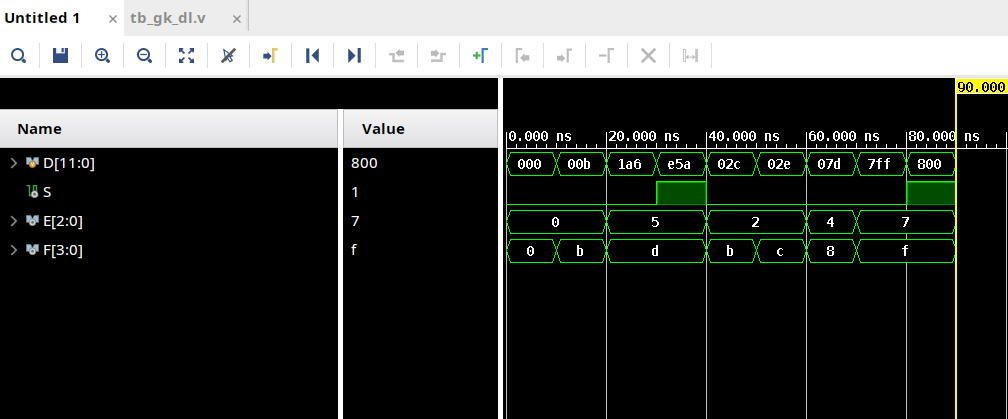
\includegraphics[width=0.80\linewidth]{image.png}
    \caption{Simulation waveform placeholder. Replace with the waveform image you want to discuss.}
    \label{fig:waveform-placeholder}
\end{figure}

\textit{Fill in:} Use this subsection to discuss the waveform evidence. Point out where the outputs match the expected results for the major test categories. If you replace the placeholder image, update the caption so it describes exactly what the figure shows.

\subsection{Bugs Found During Simulation}

\textit{Fill in:} The syllabus explicitly asks for bugs found during simulation and how they were corrected. If you encountered issues such as incorrect exponent mapping, wrong rounding direction, or mishandling of \texttt{-2048}, describe them here. If no major bug was found after your initial implementation, state that clearly and mention what you still double-checked.

\subsection{Discussion of Results}

Based on the expected values documented in the testbench, the simulation should confirm that the design behaves correctly across the main operating cases. Zero maps to \texttt{S=0, E=000, F=0000}, and the small positive input 11 maps directly to \texttt{S=0, E=000, F=1011}. The handout example 422 is encoded as \texttt{[0 101 1101]}, which expands to $13 \times 2^5 = 416$, while $-422$ produces the same exponent and significand with \texttt{S=1}. The rounding vectors show the expected split between truncation and increment, and the value 125 demonstrates the renormalization case by mapping to \texttt{[0 100 1000]}, or $8 \times 2^4 = 128$. At the upper limit, both 2047 and the approximated \texttt{-2048} case are driven to the largest available floating point encoding, showing that the design saturates as intended when exact representation is not possible.

\section{Conclusion}

\textit{Fill in:} Conclude the report by summarizing the final design, the main implementation challenges, and what you learned from the lab. The syllabus also encourages short suggestions for improving the lab, so include that here if you have any.

\section*{Appendix: Optional Code Snippets}
\addcontentsline{toc}{section}{Appendix: Optional Code Snippets}

\textit{Fill in:} If you want, include short excerpts from \texttt{FPCVT.v} here for the most important logic blocks, such as magnitude conversion, leading-zero detection, or rounding. Keep the appendix brief and only include code that you reference in the report.


\end{document}